% Material metodológico (em português, a pedido do autor) sobre duas
% alternativas de comparação de classificadores: 5x2cv com o teste F
% combinado de Alpaydin e validação cruzada K-fold repetida com o teste t
% reamostrado corrigido. Não altera o protocolo vigente
% (configs/evaluation_protocol_v4.yaml) nem executa experimentos.
% Compilação: latexmk -pdf -outdir=build main.tex
% Figuras: figuras/gerar_figuras.sh (TikZ -> PDF, SVG, PNG 600 dpi).
\documentclass[11pt,a4paper]{article}
\usepackage[T1]{fontenc}
\usepackage[utf8]{inputenc}
\usepackage[brazilian]{babel}
\usepackage[margin=2.5cm]{geometry}
\usepackage{lmodern}
\usepackage{microtype}
\usepackage{amsmath,amssymb,amsthm}
\usepackage{graphicx}
\usepackage{booktabs}
\usepackage{tabularx}
\usepackage{array}
\usepackage{enumitem}
\usepackage[table]{xcolor}
\usepackage{caption}
\usepackage{csquotes}
\usepackage[backend=biber,style=numeric-comp,sorting=none,natbib=true,
            maxbibnames=99,giveninits=true]{biblatex}
\addbibresource{referencias.bib}
\usepackage[hidelinks]{hyperref}

\setlength{\emergencystretch}{1.5em}
\captionsetup{font=small, labelfont=bf, format=plain}
\newcolumntype{L}{>{\raggedright\arraybackslash}X}
\newcommand{\tr}{\mathrm{tr}}
\newcommand{\te}{\mathrm{te}}
\newcommand{\Dtr}[1]{\mathcal{D}^{\tr}_{#1}}
\newcommand{\Dte}[1]{\mathcal{D}^{\te}_{#1}}
\newcommand{\E}{\mathbb{E}}
\newcommand{\Var}{\operatorname{Var}}
\newcommand{\MCC}{\operatorname{MCC}}

\title{Comparação estatística de classificadores:\\
validação cruzada $5\times2$ com o teste $F$ combinado e\\
validação cruzada repetida com o teste $t$ reamostrado corrigido}
\author{Lauro Moraes\\[2pt]
\small Programa de Pós-Graduação em Ciência da Computação --- UFOP\\
\small Material metodológico para a tese (projeto CapsProm)}
\date{Versão de 4 de novembro de 2026}

\begin{document}
\maketitle

\begin{abstract}
Este texto descreve duas alternativas para comparar dois algoritmos de
classificação em um mesmo conjunto de dados: a validação cruzada $5\times2$
(5$\times$2cv) com o teste $F$ combinado de \citet{alpaydin1999combined} e a
validação cruzada $K$-fold repetida $R$ vezes com o teste $t$ reamostrado
corrigido de \citet{nadeau2003inference}, na forma aplicada à validação cruzada
repetida por \citet{bouckaert2004replicability}. Separa-se o procedimento de
reamostragem do teste estatístico, distingue-se o teste $F$ combinado do teste
$\tilde t$ 5$\times$2cv de \citet{dietterich1998approximate} e indica-se qual
correção de variância corresponde à validação cruzada repetida. Discutem-se
dependência entre avaliações, custo, poder, uso do coeficiente de correlação de
Matthews (MCC), seleção de hiperparâmetros sem uso das dobras de teste,
extensão a vários conjuntos de dados e relato conjunto de significância,
magnitude de efeito e incerteza. O texto termina com uma recomendação para o
protocolo do projeto e com as condições necessárias à sua adoção. Nenhum
experimento foi executado e o protocolo vigente não foi alterado.
\end{abstract}

\tableofcontents

%======================================================================
\section{Escopo e notação}\label{sec:notacao}

O objeto de comparação é um \emph{algoritmo de aprendizagem}, isto é, o
procedimento completo que recebe um conjunto de treino e devolve um
classificador: pré-processamento ajustável, seleção de hiperparâmetros, regra
de parada, escolha de limiar, calibração e ajuste final. Os testes discutidos
aqui comparam algoritmos, e não um único modelo já ajustado
\citep{dietterich1998approximate}. O classificador que se obteria treinando no
conjunto completo não é avaliado por nenhum deles.

Seja $\mathcal{D}=\{(x_i,y_i)\}_{i=1}^{n}$ um conjunto rotulado, com
$x_i\in\Sigma^{L}$ e $y_i\in\{0,1\}$, conforme a notação canônica da tese.
Sejam $A$ e $B$ os dois algoritmos comparados e $M$ uma métrica de desempenho
em que valores maiores são melhores (por exemplo, MCC ou acurácia; para a taxa
de erro, usada por \citet{dietterich1998approximate}, basta inverter o sinal).
Uma partição de $\mathcal{D}$ em treino e teste é indexada por $(r,j)$, em que
$r=1,\dots,R$ é a repetição e $j=1,\dots,K$ a dobra. Escrevem-se
$\Dtr{rj}$ e $\Dte{rj}$ para os conjuntos de treino e de teste,
$n_{\tr}=|\Dtr{rj}|$ e $n_{\te}=|\Dte{rj}|$ (os $n_1$ e $n_2$ de
\citet{nadeau2003inference}). O desempenho do classificador produzido por $A$
a partir de $\Dtr{rj}$ e medido em $\Dte{rj}$ é $M^{A}_{rj}$, e a diferença
pareada é
\begin{equation}
  d_{rj}=M^{A}_{rj}-M^{B}_{rj}.
  \label{eq:diferenca}
\end{equation}
O pareamento é essencial: os dois algoritmos recebem exatamente o mesmo
$\Dtr{rj}$ e são avaliados exatamente no mesmo $\Dte{rj}$, de modo que a
variação comum às duas medidas se cancela na diferença.

A quantidade de interesse é a diferença esperada de desempenho de
generalização quando cada algoritmo é treinado em amostras de tamanho
$n_{\tr}$ da mesma distribuição $P$ que gerou $\mathcal{D}$:
\begin{equation}
  \mu_{n_{\tr}}=\E_{\mathcal{T}\sim P^{n_{\tr}}}\!\left[\,M\bigl(A(\mathcal{T})\bigr)-M\bigl(B(\mathcal{T})\bigr)\right],
  \label{eq:estimando}
\end{equation}
em que $M(\cdot)$ denota o desempenho esperado em novos exemplos de $P$. A
dependência de $\mu$ em relação a $n_{\tr}$ é explícita: o 5$\times$2cv
estima $\mu_{n/2}$, enquanto a validação 10-fold estima $\mu_{0{,}9n}$. As duas
alternativas, portanto, não testam exatamente a mesma hipótese
(Seção~\ref{sec:custo}).

\paragraph{Reamostragem e teste são etapas distintas.}
O \emph{procedimento de reamostragem} define como as partições
$(\Dtr{rj},\Dte{rj})$ são formadas e, assim, quantas diferenças $d_{rj}$
existem e como elas dependem entre si. O \emph{teste estatístico} é a regra
que transforma esse conjunto de diferenças em uma estatística, compara-a com
uma distribuição de referência e produz uma decisão ou um $p$-valor. A
distribuição de referência de cada teste foi deduzida, ou calibrada
empiricamente, para um esquema específico de reamostragem. A
Tabela~\ref{tab:pares} resume os pares considerados neste texto. O teste
$\tilde t$ de Dietterich e o teste $F$ de Alpaydin usam a mesma reamostragem
(5$\times$2cv) e estatísticas diferentes. O teste $t$ corrigido usa outra
reamostragem e outra lógica de correção. Trocar o teste sem trocar a
reamostragem, ou o contrário, produz um procedimento cujas propriedades não
foram estabelecidas pelas fontes originais.

\begin{table}[htbp]
\centering\small
\caption{Combinações de reamostragem e teste tratadas no texto. Cada teste
foi deduzido ou calibrado para o esquema da mesma linha. A última linha mostra
o teste ingênuo, que não deve ser usado.}
\label{tab:pares}
\begin{tabularx}{\textwidth}{@{}l l L@{}}
\toprule
Reamostragem & Teste & Fonte e observação \\
\midrule
5$\times$2cv & $\tilde t$ 5$\times$2cv, referência $t_5$ & \citet{dietterich1998approximate}; numerador com uma única diferença \\
5$\times$2cv & $F$ combinado, referência $F_{10,5}$ & \citet{alpaydin1999combined}; usa as dez diferenças \\
$R\times K$-fold & $t$ reamostrado corrigido, referência $t_{RK-1}$ & \citet{nadeau2003inference} para subamostragem aleatória; \citet{bouckaert2004replicability} para $R\times K$-fold \\
$R\times K$-fold & $t$ pareado ingênuo, referência $t_{RK-1}$ & trata as $RK$ diferenças como independentes; erro tipo I muito elevado \citep{bouckaert2004replicability} \\
\bottomrule
\end{tabularx}
\end{table}

%======================================================================
\section{\texorpdfstring{Validação cruzada 5$\times$2 e seus dois testes}{Validação cruzada 5x2 e seus dois testes}}\label{sec:5x2}

\subsection{Formação dos conjuntos de treino e de teste}

A Figura~\ref{fig:5x2cv} mostra a estrutura do procedimento. Em cada
repetição $r=1,\dots,5$, uma permutação aleatória $\pi_r$ de $\mathcal{D}$,
estratificada pela classe, divide os dados em duas metades disjuntas
$S_r^{(1)}$ e $S_r^{(2)}$, cada uma com $n/2$ exemplos. Na dobra $j=1$, cada
algoritmo é treinado em $S_r^{(1)}$ e testado em $S_r^{(2)}$; na dobra $j=2$,
os papéis se invertem \citep{dietterich1998approximate}. Cada algoritmo é
treinado $5\times2=10$ vezes, sempre com $n/2$ exemplos, e o par $(A,B)$
requer 20 ajustes finais, sem contar os ajustes da seleção interna
(Seção~\ref{sec:selecao}). O resultado são dez diferenças pareadas
$d_{rj}$, $r=1,\dots,5$, $j=1,2$.

\begin{figure}[htbp]
\centering
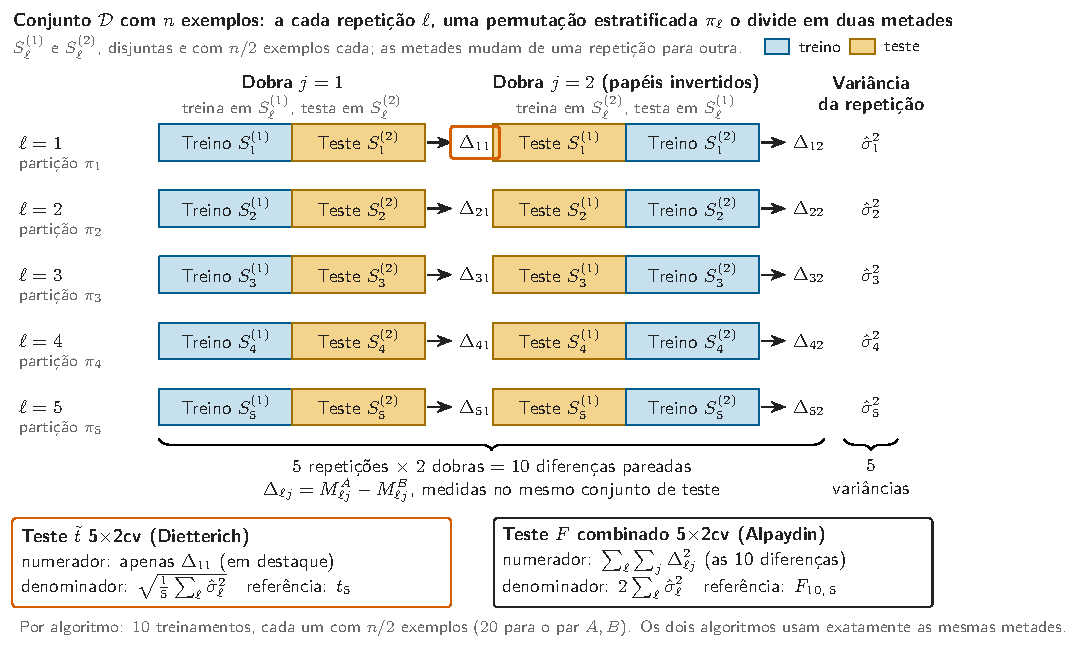
\includegraphics[width=\textwidth]{figuras/fig_5x2cv.pdf}
\caption{Estrutura da validação cruzada $5\times2$. Em cada repetição $r$,
uma permutação estratificada $\pi_r$ divide o conjunto $\mathcal{D}$ em duas
metades disjuntas $S_r^{(1)}$ e $S_r^{(2)}$ (azul: treino; laranja: teste).
Na dobra $j=1$ treina-se em $S_r^{(1)}$ e testa-se em $S_r^{(2)}$; na dobra
$j=2$ os papéis se invertem. Cada dobra produz uma diferença pareada
$d_{rj}=M^{A}_{rj}-M^{B}_{rj}$, calculada no mesmo conjunto de teste para os
dois algoritmos, e cada repetição produz uma variância $s_r^{2}$. O teste
$\tilde t$ de \citet{dietterich1998approximate} usa apenas $d_{11}$ (em
destaque) no numerador; o teste $F$ combinado de
\citet{alpaydin1999combined} usa as dez diferenças. Esquema estrutural, sem
valores numéricos.}
\label{fig:5x2cv}
\end{figure}

Para cada repetição definem-se a média e a variância das duas diferenças:
\begin{equation}
  \bar d_r=\frac{d_{r1}+d_{r2}}{2},\qquad
  s_r^{2}=(d_{r1}-\bar d_r)^2+(d_{r2}-\bar d_r)^2=\frac{(d_{r1}-d_{r2})^2}{2}.
  \label{eq:sr2}
\end{equation}
Na notação original, $d_{rj}$ corresponde a $p_i^{(j)}$, com $i$ no lugar de
$r$ e a diferença de taxas de erro no lugar da diferença de métricas
\citep{dietterich1998approximate,alpaydin1999combined}. A letra $r$ é usada
aqui porque $i$ indexa exemplos na tese.

\subsection{Hipóteses}

Os dois testes avaliam
\begin{equation}
  H_0:\ \mu_{n/2}=0
  \qquad\text{contra}\qquad
  H_1:\ \mu_{n/2}\neq0,
  \label{eq:hipoteses5x2}
\end{equation}
ou seja, se os dois algoritmos, treinados com metade dos dados, têm o mesmo
desempenho esperado. As duas hipóteses são bilaterais.

\subsection{\texorpdfstring{Teste $\tilde t$ 5$\times$2cv de Dietterich}{Teste t 5x2cv de Dietterich}}

\citet{dietterich1998approximate} define
\begin{equation}
  \tilde t=\frac{d_{11}}{\sqrt{\tfrac15\sum_{r=1}^{5}s_r^{2}}},
  \label{eq:dietterich}
\end{equation}
que, sob $H_0$, segue aproximadamente uma distribuição $t$ de Student com 5
graus de liberdade. Rejeita-se $H_0$ ao nível $\alpha$ quando
$|\tilde t|>t_{5;\,1-\alpha/2}$ (2,571 para $\alpha=0{,}05$). O numerador usa
somente a primeira diferença da primeira repetição. Segundo o autor,
substituir o numerador pela média das diferenças tornava a estatística
instável, porque a média é mal estimada quando as dobras são correlacionadas.
A dedução assume que $d_{11}/\sigma$ é aproximadamente normal padrão (o que
requer conjuntos de teste com pelo menos cerca de 30 exemplos), que
$d_{r1}$ e $d_{r2}$ são independentes, de modo que $s_r^2/\sigma^2\sim\chi^2_1$,
que os $s_r^2$ são independentes entre repetições, de modo que
$\sum_r s_r^2/\sigma^2\sim\chi^2_5$, e que numerador e denominador são
independentes. O próprio autor afirma que essas hipóteses de independência são
violadas e que o teste é heurístico, validado por simulação; o número de cinco
repetições foi escolhido empiricamente \citep{dietterich1998approximate}.

\subsection{\texorpdfstring{Teste $F$ combinado 5$\times$2cv de Alpaydin}{Teste F combinado 5x2cv de Alpaydin}}

\citet{alpaydin1999combined} observou que a escolha de $d_{11}$ é arbitrária:
qualquer uma das dez diferenças poderia ocupar o numerador, e a simples
reordenação das repetições ou das dobras muda o resultado do teste $\tilde t$.
A proposta combina as dez estatísticas. Sob $H_0$, se $d_{rj}/\sigma\sim
\mathcal{N}(0,1)$, então
\begin{equation}
  N=\frac{\sum_{r=1}^{5}\sum_{j=1}^{2}d_{rj}^{2}}{\sigma^{2}}\sim\chi^{2}_{10},
  \qquad
  M=\frac{\sum_{r=1}^{5}s_r^{2}}{\sigma^{2}}\sim\chi^{2}_{5},
\end{equation}
e a razão entre as duas variáveis, cada uma dividida por seus graus de
liberdade, define
\begin{equation}
  f=\frac{N/10}{M/5}=\frac{\sum_{r=1}^{5}\sum_{j=1}^{2}d_{rj}^{2}}{2\sum_{r=1}^{5}s_r^{2}},
  \label{eq:alpaydin}
\end{equation}
aproximadamente distribuída como $F$ com 10 e 5 graus de liberdade. Rejeita-se
$H_0$ ao nível $\alpha$ quando $f>F_{10,5;\,1-\alpha}$ (4,74 para
$\alpha=0{,}05$). A estatística depende das diferenças apenas por seus
quadrados. A rejeição indica que os algoritmos diferem, mas o teste não
informa qual deles é melhor; a direção é lida no sinal de $\bar d=\frac1{10}
\sum_{r,j}d_{rj}$. As hipóteses de normalidade e independência são as mesmas
de Dietterich, acrescidas da independência entre $N$ e $M$, que também é
apenas aproximada. Nas simulações do autor, a versão combinada teve erro tipo
I menor e poder maior que o teste $\tilde t$ \citep{alpaydin1999combined}.

\subsection{Diferenças entre os dois testes}

Os dois testes compartilham a reamostragem, o denominador baseado em
$\sum_r s_r^2$ e as hipóteses distribucionais. Eles diferem no numerador
($d_{11}$ contra a soma dos dez quadrados), na distribuição de referência
($t_5$ contra $F_{10,5}$), na direcionalidade (o $\tilde t$ tem sinal; o $f$
não) e na estabilidade diante da ordem das repetições. Os valores críticos
2,571 e 4,74 não são intercambiáveis e um não é uma transformação do outro.
Também não é correto calcular $f$ a partir de outro esquema de reamostragem:
os graus de liberdade 10 e 5 vêm da estrutura de cinco repetições com duas
dobras disjuntas, em que cada $s_r^2$ tem um grau de liberdade.

%======================================================================
\section{\texorpdfstring{Validação cruzada repetida e o teste $t$ corrigido}{Validação cruzada repetida e o teste t corrigido}}\label{sec:rkcv}

\subsection{Formação dos conjuntos de treino e de teste}

A Figura~\ref{fig:kfold} mostra a validação cruzada $K$-fold repetida $R$
vezes. Em cada repetição $r$, uma nova permutação estratificada $\pi_r$
divide $\mathcal{D}$ em $K$ subconjuntos disjuntos $F_{r,1},\dots,F_{r,K}$. Na
dobra $j$, o conjunto de teste é $\Dte{rj}=F_{r,j}$ e o de treino é a união
dos demais, de modo que $n_{\te}\approx n/K$ e $n_{\tr}\approx n(K-1)/K$. Cada
algoritmo é treinado $RK$ vezes; com $R=K=10$, são 100 ajustes finais por
algoritmo e 200 para o par. Os dois algoritmos usam as mesmas permutações e as
mesmas dobras, e o resultado são $J=RK$ diferenças pareadas $d_{rj}$.

\begin{figure}[htbp]
\centering
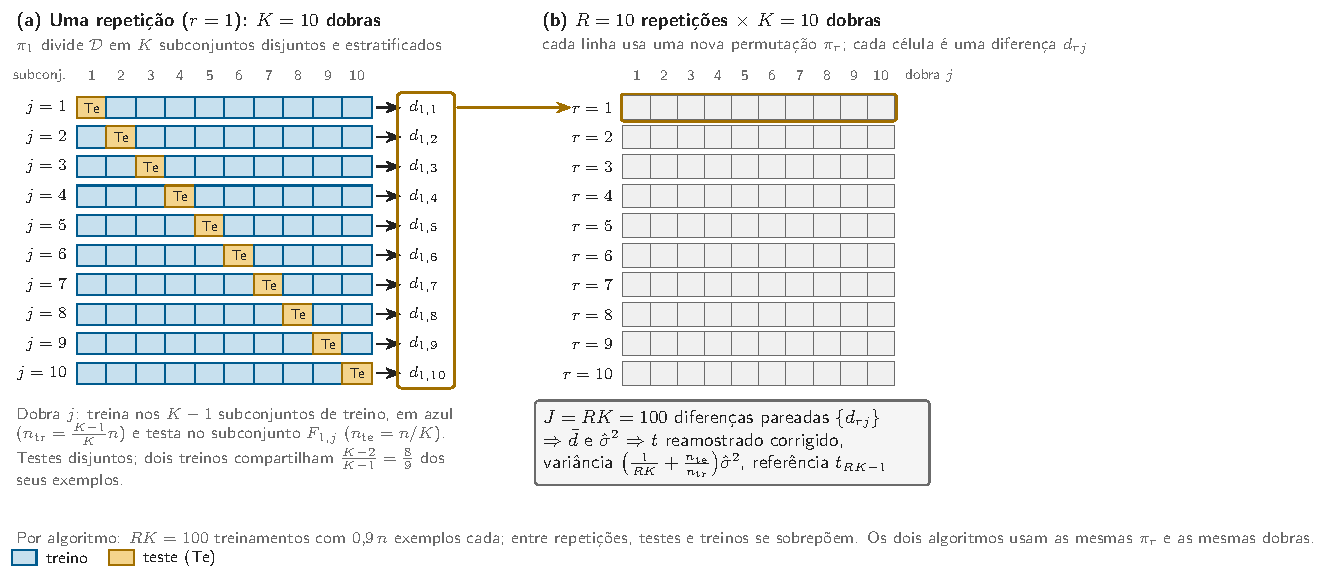
\includegraphics[width=\textwidth]{figuras/fig_kfold_repetido.pdf}
\caption{Estrutura da validação cruzada $K$-fold repetida $R$ vezes, com
$R=K=10$. (a) Em uma repetição, a permutação estratificada $\pi_1$ divide
$\mathcal{D}$ em $K$ subconjuntos disjuntos; na dobra $j$, o subconjunto $j$
é o teste (laranja, ``Te'') e os outros $K-1$ formam o treino (azul). Cada
dobra produz uma diferença pareada $d_{1,j}$. (b) Cada linha da grade é uma
repetição com nova permutação $\pi_r$ e cada célula é uma diferença $d_{rj}$
obtida com os mesmos treino e teste para os dois algoritmos; a linha
destacada corresponde ao painel (a). As $RK$ diferenças alimentam o teste $t$
reamostrado corrigido \citep{nadeau2003inference,bouckaert2004replicability}.
Esquema estrutural, sem valores numéricos.}
\label{fig:kfold}
\end{figure}

\subsection{\texorpdfstring{Por que o teste $t$ ingênuo falha}{Por que o teste t ingênuo falha}}

Com $\bar d=\frac{1}{RK}\sum_{r=1}^{R}\sum_{j=1}^{K}d_{rj}$ e
$\hat\sigma^{2}=\frac{1}{RK-1}\sum_{r,j}(d_{rj}-\bar d)^2$, o teste pareado
usual usaria $\bar d/\sqrt{\hat\sigma^2/(RK)}$ com $RK-1$ graus de liberdade.
Essa estatística supõe diferenças independentes. Elas não o são: dentro de uma
repetição, os conjuntos de teste são disjuntos, mas dois conjuntos de treino
compartilham uma fração $(K-2)/(K-1)$ dos seus exemplos (8/9 para $K=10$);
entre repetições, treinos e testes se sobrepõem. A variância de $\bar d$ é,
assim, subestimada e o erro tipo I é muito superior ao nominal
\citep{dietterich1998approximate,bouckaert2004replicability}.

\subsection{A correção de Nadeau e Bengio}

\citet{nadeau2003inference} consideram $J$ estimativas com variância comum
$\sigma^2$ e correlação comum $\rho$ entre pares. Nessas condições,
\begin{equation}
  \Var(\bar d)=\sigma^{2}\Bigl(\rho+\frac{1-\rho}{J}\Bigr),
  \qquad
  \E[\hat\sigma^{2}]=\sigma^{2}(1-\rho),
\end{equation}
de modo que $\bigl(\frac1J+\frac{\rho}{1-\rho}\bigr)\hat\sigma^{2}$ é um
estimador não viesado de $\Var(\bar d)$. Como $\rho$ é desconhecida e difícil
de estimar, os autores adotam o substituto $\rho_0=n_{\te}/n$, obtido sob a
aproximação de que a perda em um exemplo de teste depende apenas desse
exemplo e de $n_{\tr}$, e não do conjunto de treino específico. Como
$\rho_0/(1-\rho_0)=n_{\te}/n_{\tr}$, a estatística corrigida para a validação
cruzada repetida \citep{bouckaert2004replicability} é
\begin{equation}
  t_c=\frac{\bar d}{\sqrt{\Bigl(\dfrac{1}{RK}+\dfrac{n_{\te}}{n_{\tr}}\Bigr)\hat\sigma^{2}}},
  \qquad
  \frac{n_{\te}}{n_{\tr}}=\frac{1}{K-1}\ \text{para dobras de tamanho igual},
  \label{eq:tcorrigido}
\end{equation}
comparada com a distribuição $t$ com $RK-1$ graus de liberdade. As hipóteses
são $H_0:\mu_{n_{\tr}}=0$ contra $H_1:\mu_{n_{\tr}}\neq0$, e rejeita-se $H_0$
quando $|t_c|>t_{RK-1;\,1-\alpha/2}$. Com $R=K=10$, o fator de variância passa
de $1/100=0{,}01$ (teste ingênuo) para $1/100+1/9\approx0{,}121$; a variância
estimada de $\bar d$ é multiplicada por cerca de 12,1 e o erro-padrão por
cerca de 3,5.

\citet{bouckaert2004replicability} chamam essa forma de \emph{corrected
repeated $k$-fold cv test}: justificam a aplicação da correção observando que
a validação cruzada é um caso particular da subamostragem aleatória em que os
testes de uma mesma repetição não se sobrepõem. Em seus experimentos, a
replicabilidade, isto é, a concordância do resultado do teste entre diferentes
particionamentos aleatórios dos mesmos dados, foi boa com 100 subamostragens e
o teste corrigido, e melhor ainda com $10\times10$-fold, configuração que
recomendam.

\paragraph{Limites da correção.}
A correção é heurística. O substituto $\rho_0$ pode subestimar ou superestimar
a correlação verdadeira e, portanto, a variância \citep{nadeau2003inference};
além disso, não existe estimador não viesado da variância da validação cruzada
$K$-fold que seja válido para qualquer distribuição \citep{bengio2004noUnbiased}.
O lema também supõe uma correlação única para todos os pares de diferenças,
enquanto na validação repetida os pares da mesma repetição e de repetições
distintas se correlacionam de formas diferentes. Os $RK-1$ graus de liberdade
são nominais: quando $J\to\infty$, $\Var(\bar d)\to\rho\sigma^{2}$, ou seja,
aumentar $R$ reduz o ruído devido à escolha das partições e melhora a
replicabilidade, mas não cria informação nova sobre $P$. A correção foi
proposta para $n_{\tr}$ bem maior que $n_{\te}$; os autores observam que o uso
normal teria $n_{\tr}$ cinco a dez vezes maior que $n_{\te}$
\citep{nadeau2003inference}. Aplicá-la ao 5$\times$2cv, em que
$n_{\te}/n_{\tr}=1$, não é o procedimento avaliado pelas fontes; aplicar o teste
$F$ de Alpaydin à validação $10\times10$ também não é, porque sua distribuição
de referência depende da estrutura com duas dobras.

\paragraph{Alternativa bayesiana.}
O teste $t$ bayesiano correlacionado de \citet{corani2015bayesian} usa a mesma
correlação $\rho_0=n_{\te}/n$ e produz uma distribuição \emph{a posteriori}
para $\mu_{n_{\tr}}$. Com uma região de equivalência prática (ROPE), ele
responde diretamente a perguntas como ``qual a probabilidade de $A$ superar
$B$ por mais que um limiar relevante?'' \citep{benavoli2017timeforchange}. As
hipóteses sobre a correlação permanecem as mesmas.

%======================================================================
\section{Dependência entre avaliações}\label{sec:dependencia}

A Tabela~\ref{tab:dependencia} separa as fontes de dependência e a forma como
cada procedimento as trata. O pareamento, isto é, a avaliação de $A$ e $B$ no
mesmo teste, é uma dependência desejada, pois reduz a variância da
diferença. As demais são problemas a corrigir.

\begin{table}[htbp]
\centering\small
\caption{Fontes de dependência entre as diferenças pareadas e o tratamento
dado por cada procedimento. Nenhum dos testes trata a dependência entre
exemplos; ela precisa ser resolvida na construção das partições.}
\label{tab:dependencia}
\begin{tabularx}{\textwidth}{@{}L L L@{}}
\toprule
Fonte & 5$\times$2cv ($\tilde t$ e $F$) & $R\times K$-fold com $t_c$ \\
\midrule
Mesmo teste para $A$ e $B$ & desejada; anulada na diferença $d_{rj}$ & desejada; anulada na diferença $d_{rj}$ \\
Dobras da mesma repetição & treinos disjuntos, mas o treino de uma dobra é o teste da outra; independência assumida & testes disjuntos, treinos compartilham $(K-2)/(K-1)$; coberta por $\rho_0$ \\
Repetições distintas & mesmos dados reparticionados; independência dos $s_r^2$ assumida & treinos e testes sobrepostos; coberta por $\rho_0$ \\
Variação do algoritmo (semente) & entra em $s_r^2$ se cada ajuste tiver semente própria & entra em $\hat\sigma^2$ se cada ajuste tiver semente própria \\
Exemplos dependentes (homologia, janelas sobrepostas) & não tratada; exige metades por grupo & não tratada; exige dobras por grupo \\
\bottomrule
\end{tabularx}
\end{table}

O 5$\times$2cv usa duas dobras porque nelas os conjuntos de treino são
disjuntos, o que torna a hipótese de independência entre $d_{r1}$ e $d_{r2}$
menos irrealista; mesmo assim, o treino de uma dobra é o teste da outra, e as
cinco repetições reusam os mesmos dados \citep{dietterich1998approximate}. O
teste $F$ não modela essas dependências: ele reduz a instabilidade do
numerador, mas mantém as hipóteses de independência. O teste $t_c$ não assume
independência; modela-a por uma correlação única e aproximada. Todos os
procedimentos supõem exemplos independentes e identicamente distribuídos.
Quando há sequências homólogas ou janelas sobrepostas, partições aleatórias
por exemplo colocam exemplos dependentes em treino e teste, inflam o
desempenho medido e tornam a correção insuficiente; as partições devem ser
feitas por grupo \citep{roberts2017crossvalidation}. Com grupos, $n_{\te}$
varia entre dobras, e a razão $n_{\te}/n_{\tr}$ em \eqref{eq:tcorrigido} deve
ser a média registrada no manifesto de partições.

%======================================================================
\section{Custo, poder, limitações e uso do MCC}\label{sec:custo}

\paragraph{Custo computacional.}
Com $H$ configurações de hiperparâmetros avaliadas por validação cruzada
interna de $I$ dobras, cada ajuste externo exige $IH+1$ treinamentos. O
5$\times$2cv requer $10(IH+1)$ treinamentos por algoritmo, com $n/2$ exemplos;
a validação $10\times10$ requer $100(IH+1)$, com $0{,}9n$ exemplos. Para redes
neurais, que podem custar ordens de grandeza mais que modelos lineares, essa
diferença de dez vezes, multiplicada pelo número de conjuntos de dados, pode
decidir a viabilidade.

\paragraph{Poder e calibração.}
Nas simulações de \citet{dietterich1998approximate}, o $\tilde t$ teve erro
tipo I igual ou inferior ao nominal e poder menor que o do teste $t$ da
validação 10-fold, que por sua vez teve erro tipo I elevado. O teste $F$
combinado teve erro tipo I menor e poder maior que o $\tilde t$
\citep{alpaydin1999combined}. O teste corrigido teve erro tipo I próximo do
nominal sem a perda de poder do 5$\times$2cv \citep{nadeau2003inference} e
a melhor replicabilidade na configuração $10\times10$
\citep{bouckaert2004replicability}, que, no entanto, não avaliaram o teste $F$
combinado. Com apenas cinco graus de liberdade no denominador, o 5$\times$2cv
tende a ser conservador: diferenças pequenas, mas reais, frequentemente não
são detectadas.

\paragraph{Tamanho do treino.}
O 5$\times$2cv treina com metade dos dados. Quando o desempenho ainda cresce
com o tamanho da amostra, a estimativa é pessimista \citep{efron1997improvements}
e, como as curvas de aprendizagem diferem entre famílias de modelos, o viés
pode ser diferente para $A$ e $B$. Uma rede neural profunda e um modelo linear
podem trocar de posição entre $n/2$ e $0{,}9n$ exemplos: nesse caso, os dois
procedimentos respondem a perguntas diferentes, $\mu_{n/2}$ e $\mu_{0{,}9n}$.

\paragraph{Uso do MCC.}
O coeficiente de correlação de Matthews \citep{matthews1975comparison},
\begin{equation}
  \MCC=\frac{TP\cdot TN-FP\cdot FN}{\sqrt{(TP+FP)(TP+FN)(TN+FP)(TN+FN)}},
\end{equation}
usa as quatro células da matriz de confusão e é informativo sob
desbalanceamento \citep{chicco2020mcc}. Os testes discutidos foram deduzidos
para diferenças de taxas de erro, cuja normalidade aproximada vem da
aproximação normal da binomial. Para o MCC, a normalidade das diferenças por
dobra é uma aproximação assintótica adicional, pior em dobras pequenas e com
poucos positivos, situação mais frequente na validação 10-fold. Quatro
cuidados são necessários. Primeiro, o MCC deve ser calculado em cada dobra,
gerando um $d_{rj}$ por dobra; o MCC agregado das predições fora da dobra não
fornece as diferenças por partição exigidas pelas estatísticas
\eqref{eq:alpaydin} e \eqref{eq:tcorrigido}. Segundo, o MCC é indefinido
quando alguma soma do denominador é nula, por exemplo, quando um classificador
prediz uma única classe em uma dobra; a convenção adotada nesses casos deve ser
fixada antes da execução e cada ocorrência deve ser relatada. Terceiro, a
estratificação deve garantir um número mínimo de exemplos de cada classe por
dobra de teste. Quarto, o MCC depende do limiar, que precisa ser fixado sem o
teste (Seção~\ref{sec:selecao}).

%======================================================================
\section{Seleção sem uso das dobras de teste}\label{sec:selecao}

A Figura~\ref{fig:fluxo} mostra o fluxo completo de uma comparação. A
validação externa só estima o desempenho do algoritmo se cada dobra de teste
for usada apenas para medir o desempenho do classificador já ajustado. Toda
decisão que aprende com dados é parte do algoritmo e deve ser refeita dentro
de cada $\Dtr{rj}$:
\begin{itemize}[leftmargin=*]
  \item \textbf{Hiperparâmetros:} escolhidos por validação cruzada interna em
    $\Dtr{rj}$ (validação aninhada). Selecionar hiperparâmetros com as mesmas
    dobras usadas para estimar o desempenho produz estimativas otimistas
    \citep{varma2006bias,cawley2010overfitting}. O espaço de busca e o
    orçamento devem ser fixados de antemão e ser equivalentes para $A$ e $B$.
  \item \textbf{\emph{Early stopping} e número de épocas:} definidos em
    subconjuntos de validação extraídos de $\Dtr{rj}$; para o ajuste final no
    treino completo, usa-se uma regra prefixada, como a mediana das épocas
    ótimas das dobras internas.
  \item \textbf{Limiar e calibração:} um limiar fixo, como 0,5, ou um limiar
    escolhido por predições fora da dobra interna; o calibrador é ajustado nas
    mesmas predições internas.
  \item \textbf{Pré-processamento ajustável:} padronização, seleção de
    atributos e vocabulários são ajustados em $\Dtr{rj}$ e aplicados a
    $\Dte{rj}$.
  \item \textbf{Partições internas:} respeitam os mesmos grupos de
    dependência das partições externas.
\end{itemize}

\begin{figure}[htbp]
\centering
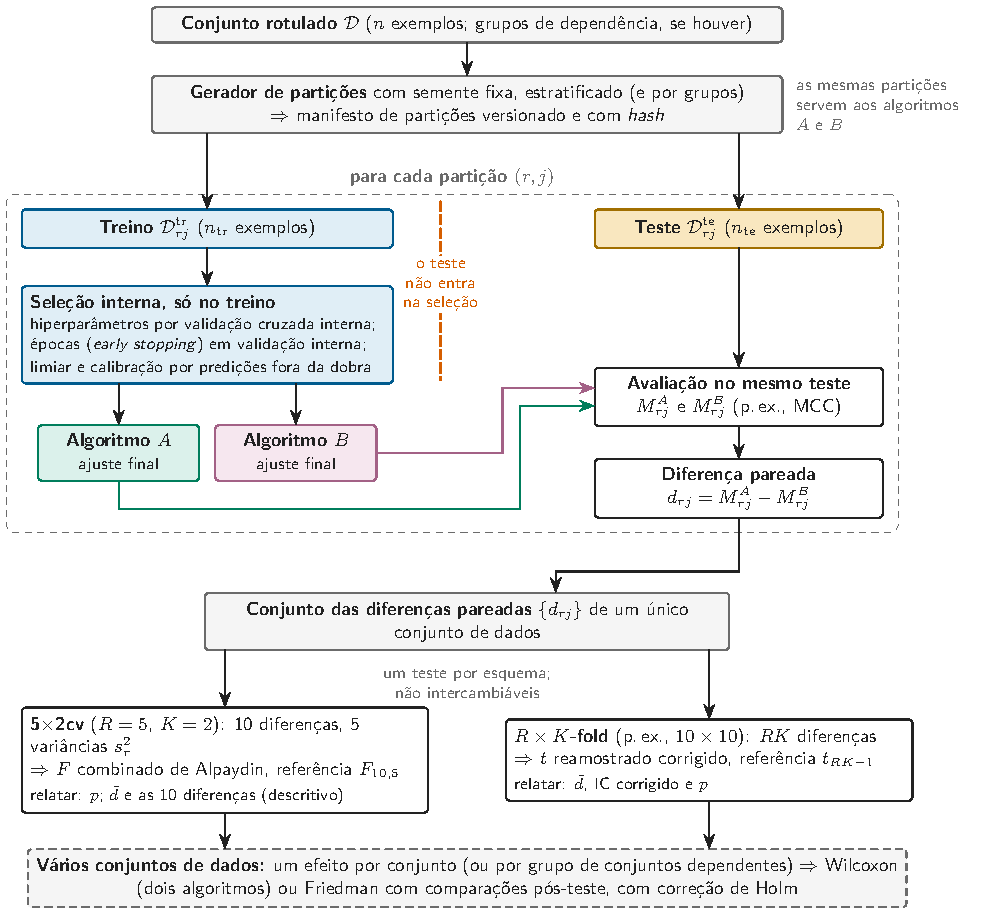
\includegraphics[width=\textwidth]{figuras/fig_fluxo_comparacao.pdf}
\caption{Fluxo da comparação estatística pareada entre os algoritmos $A$ e
$B$. Um gerador de partições com semente fixa produz um manifesto único,
usado pelos dois algoritmos. Em cada partição $(r,j)$, a seleção de
hiperparâmetros, épocas, limiar e calibração ocorre apenas no treino; a linha
tracejada vermelha indica que o teste não alimenta essa seleção. Os dois
classificadores ajustados são avaliados no mesmo teste, gerando
$d_{rj}=M^{A}_{rj}-M^{B}_{rj}$. O conjunto das diferenças segue para o teste
correspondente ao esquema de reamostragem: $F$ combinado para 5$\times$2cv e
$t$ reamostrado corrigido para $R\times K$-fold. Comparações em vários
conjuntos de dados usam um efeito por conjunto (ou por grupo de conjuntos
dependentes). Esquema estrutural, sem valores numéricos.}
\label{fig:fluxo}
\end{figure}

Além disso, o desenho do experimento, as métricas, o número de repetições, as
sementes e a convenção para valores indefinidos devem ser declarados antes da
execução. Repetir a comparação com novas partições ou sementes até obter
significância invalida o nível nominal do teste, e qualquer análise decidida
depois de ver os resultados deve ser rotulada como exploratória.

%======================================================================
\section{Um conjunto de dados ou vários}\label{sec:multiplos}

Os testes das Seções~\ref{sec:5x2} e~\ref{sec:rkcv} respondem a uma pergunta
condicionada a um conjunto de dados: se, na distribuição que gerou
$\mathcal{D}$ e com treinos de tamanho $n_{\tr}$, os algoritmos diferem. Eles
não informam se a diferença se repete em outros domínios, organismos ou
fontes de dados. As variâncias $s_r^2$ e $\hat\sigma^2$ medem a variação devida
ao treino, ao teste e à semente dentro de uma distribuição, e não a variação
entre distribuições.

Para afirmar que um algoritmo é melhor em geral, a unidade amostral passa a
ser o conjunto de dados. \citet{demsar2006statistical} recomenda o teste de
postos sinalizados de Wilcoxon sobre um efeito por conjunto para dois
algoritmos e o teste de Friedman, seguido de comparações pós-teste, para vários
algoritmos. \citet{garcia2008extension} propõem procedimentos pós-teste mais
poderosos, e \citet{benavoli2016posthoc} desaconselham pós-testes baseados em
postos médios, que dependem dos demais algoritmos incluídos, em favor de
comparações pareadas com correção de multiplicidade. Conjuntos derivados da
mesma fonte não são independentes; devem ser agrupados, contribuindo com um
único efeito, para não inflar o tamanho amostral efetivo. No enfoque
bayesiano, \citet{corani2015bayesian} combinam o teste correlacionado de cada
conjunto com uma análise entre conjuntos, e \citet{benavoli2017timeforchange}
discutem modelos hierárquicos que tratam ao mesmo tempo a variação dentro de
cada conjunto, com a correlação $\rho_0$, e entre conjuntos.

O tratamento de comparações múltiplas é necessário em três situações:
\begin{enumerate}[leftmargin=*]
  \item quando um teste por conjunto de dados é aplicado a muitos conjuntos e
    as conclusões são enunciadas conjunto a conjunto (com 18 conjuntos e
    $\alpha=0{,}05$, a probabilidade de ao menos um falso positivo sob $H_0$
    global chega a $1-0{,}95^{18}\approx0{,}60$ se os testes forem
    independentes);
  \item quando há mais de dois algoritmos, ou vários pares de interesse;
  \item quando várias métricas são usadas para sustentar a mesma alegação.
\end{enumerate}
A correção de \citet{holm1979simple} controla a taxa de erro por família de
hipóteses e rejeita, no mínimo, as mesmas hipóteses que a correção de
Bonferroni. Contar quantos
conjuntos de dados tiveram diferença ``significativa'' não é um teste válido
entre conjuntos \citep{demsar2006statistical}.

%======================================================================
\section{Significância, magnitude do efeito e incerteza}\label{sec:efeito}

Um $p$-valor não mede o tamanho do efeito nem sua importância
\citep{wasserstein2016asa}. Cada análise deve relatar a estimativa do efeito, na
escala da métrica, sua incerteza e, só então, o resultado do teste. O que é
justificável depende do procedimento:
\begin{itemize}[leftmargin=*]
  \item \textbf{5$\times$2cv com $F$ combinado:} $p$-valor de $F_{10,5}$;
    $\bar d$ e as dez diferenças como descrição. A construção não fornece um
    intervalo de confiança para $\mu_{n/2}$, porque a estatística é não
    direcional. O $\tilde t$ de Dietterich permitiria um intervalo centrado em
    $d_{11}$, mas ele herda a instabilidade do numerador e não é
    recomendado.
  \item \textbf{$R\times K$-fold com $t_c$:} $\bar d$ com o intervalo
    \begin{equation}
      \bar d\pm t_{RK-1;\,1-\alpha/2}\sqrt{\Bigl(\frac{1}{RK}+\frac{n_{\te}}{n_{\tr}}\Bigr)\hat\sigma^{2}},
      \label{eq:ic}
    \end{equation}
    válido sob as mesmas aproximações do teste; o $p$-valor é coerente com o
    intervalo.
  \item \textbf{Abordagem bayesiana correlacionada:} distribuição
    \emph{a posteriori} de $\mu_{n_{\tr}}$, intervalo de credibilidade e
    probabilidades de superioridade, equivalência prática e inferioridade em
    relação a uma ROPE prefixada.
  \item \textbf{Vários conjuntos de dados:} mediana das diferenças por
    conjunto (ou por grupo de conjuntos), intervalo obtido pela inversão do
    teste de Wilcoxon ou por \emph{bootstrap} por grupo
    \citep{field2007bootstrapping}, e $p$-valores ajustados por Holm.
\end{itemize}
Quando a métrica primária é o MCC, a diferença $\Delta\MCC$ deve ser
interpretada diante de um limiar de relevância prática fixado antes da
análise. Uma diferença estatisticamente significativa e menor que esse limiar
não sustenta superioridade prática; uma diferença não significativa com
intervalo largo indica falta de precisão, não equivalência.

%======================================================================
\section{Tabela comparativa}\label{sec:tabela}

A Tabela~\ref{tab:comparativa} reúne as propriedades discutidas nas seções
anteriores.

\begin{table}[htbp]
\centering\small
\caption{Comparação dos procedimentos. As propriedades de erro tipo I, poder e
replicabilidade vêm das simulações das fontes citadas, com taxas de erro como
métrica, e não foram verificadas para o MCC.}
\label{tab:comparativa}
\renewcommand{\arraystretch}{1.12}
\begin{tabularx}{\textwidth}{@{}>{\raggedright\arraybackslash}p{2.9cm} L L L@{}}
\toprule
 & 5$\times$2cv + $\tilde t$ \citep{dietterich1998approximate} & 5$\times$2cv + $F$ combinado \citep{alpaydin1999combined} & $R\times K$-fold + $t_c$ \citep{nadeau2003inference,bouckaert2004replicability} \\
\midrule
Partições & 5 repetições, 2 metades & 5 repetições, 2 metades & $R$ repetições, $K$ dobras (p.\,ex., $10\times10$) \\
Ajustes por algoritmo & 10 & 10 & $RK$ (100) \\
$n_{\tr}$ / $n_{\te}$ & $n/2$ / $n/2$ & $n/2$ / $n/2$ & $\tfrac{K-1}{K}n$ / $n/K$ \\
Diferenças usadas & $d_{11}$ e os 5 $s_r^2$ & 10 $d_{rj}$ e os 5 $s_r^2$ & $RK$ $d_{rj}$ \\
Estatística & \eqref{eq:dietterich} & \eqref{eq:alpaydin} & \eqref{eq:tcorrigido} \\
Referência & $t_5$ & $F_{10,5}$ & $t_{RK-1}$ (nominal) \\
Direção & bilateral, com sinal & sem sinal (direção por $\bar d$) & bilateral, com sinal \\
Dependência & independências assumidas & independências assumidas & correlação $\rho_0=n_{\te}/n$ \\
Intervalo para o efeito & centrado em $d_{11}$; instável & não fornecido & \eqref{eq:ic} \\
Erro tipo I & $\le$ nominal & menor que o $\tilde t$ & próximo do nominal \\
Poder & baixo & maior que o $\tilde t$ & maior que o 5$\times$2cv \\
Replicabilidade & baixa (depende de $d_{11}$) & maior que o $\tilde t$ (combina as 10) & a melhor entre os avaliados ($10\times10$) \\
Custo relativo & $1\times$ & $1\times$ & $\approx10\times$ \\
Principais riscos & arbitrariedade do numerador; treino com $n/2$ & treino com $n/2$; sem intervalo; 5 g.l. & correção heurística; g.l. nominais; dobras pequenas para o MCC \\
\bottomrule
\end{tabularx}
\end{table}

%======================================================================
\section{Recomendação para o protocolo do projeto}\label{sec:recomendacao}

O protocolo confirmatório vigente do CapsProm
(\path{specs/statistical_evaluation_protocol.md} e
\path{configs/evaluation_protocol_v4.yaml}) avalia cada conjunto de dados
em uma partição de teste fixa, usada uma única vez depois que a configuração é
congelada. Ele seleciona modelos por validação cruzada interna de cinco dobras,
estratificada e agrupada por homologia; repete os modelos estocásticos com dez
sementes prefixadas; mede a incerteza por \emph{bootstrap} pareado por grupo de
homologia; e faz a inferência entre conjuntos com Wilcoxon ou Friedman sobre
grupos de dependência auditados, com correção de Holm. Esse desenho não usa
nenhuma das duas alternativas discutidas aqui. A recomendação a seguir não
altera esse protocolo.

\paragraph{Recomendação.}
Manter o desenho vigente como análise primária. Se o projeto precisar de uma
inferência por conjunto de dados que incorpore a variação devida à escolha do
conjunto de treino, que a partição fixa e o \emph{bootstrap} do teste não
medem, a alternativa preferível é a validação cruzada $10\times10$,
estratificada e agrupada por homologia, com o teste $t$ reamostrado corrigido
\eqref{eq:tcorrigido}, relatando $\overline{\Delta\MCC}$ com o intervalo
\eqref{eq:ic}, como análise secundária predeclarada. Três razões sustentam essa
escolha: (i) a estimativa refere-se a treinos com $0{,}9$ do conjunto de
desenvolvimento, e não à metade dele, o que importa para comparar redes de
cápsulas com modelos lineares, cujas curvas de aprendizagem podem diferir; (ii)
o procedimento fornece um intervalo para o efeito, e não apenas um $p$-valor;
(iii) entre os procedimentos avaliados, teve a melhor replicabilidade
\citep{bouckaert2004replicability}. O 5$\times$2cv com o teste $F$ combinado
fica como alternativa apenas quando o custo da validação aninhada $10\times10$
for inviável para as redes neurais; nesse caso, deve-se declarar que a
hipótese testada é $\mu_{n/2}$ e que o resultado não traz intervalo para o
efeito. O teste $\tilde t$ de Dietterich não é recomendado, pois o $F$
combinado o substitui com a mesma reamostragem e o mesmo custo.

\paragraph{Condições necessárias à adoção.}
\begin{enumerate}[leftmargin=*]
  \item \textbf{Nova versão do contrato.} A análise exige uma nova
    configuração versionada de avaliação e um novo caminho de estado, criados e
    congelados antes de qualquer execução, conforme as regras do repositório.
    A versão 4 e seus resultados permanecem intactos.
  \item \textbf{Partição de teste preservada.} A validação repetida deve
    ocorrer apenas na partição de treino de cada conjunto. Reparticionar treino
    e teste juntos consumiria a partição reservada e romperia a regra de uso
    único e a comparabilidade com as partições publicadas.
  \item \textbf{Seleção refeita em cada dobra externa.} A configuração
    congelada da versão 4 foi escolhida com toda a partição de treino; reusá-la
    nas dobras externas faria cada dobra de teste participar da seleção. Cada
    dobra externa deve repetir a seleção interna (hiperparâmetros, regra de
    épocas, limiar e calibração), com o mesmo espaço de busca e o mesmo
    orçamento para todos os algoritmos.
  \item \textbf{Partições agrupadas e registradas.} As partições externas e
    internas devem respeitar os grupos de homologia e a estratificação por
    classe, gerar um manifesto com \emph{hash} idêntico para todos os
    algoritmos e registrar $n_{\te}$ e $n_{\tr}$ de cada dobra, para o cálculo
    de $n_{\te}/n_{\tr}$ médio.
  \item \textbf{Sementes prefixadas.} A atribuição de sementes às $RK$
    execuções deve ser fixada na política de sementes antes da execução.
    Execuções que falharem são relatadas e não substituídas.
  \item \textbf{MCC por dobra com regras prefixadas.} Deve-se fixar o
    tamanho mínimo de cada classe por dobra de teste, a convenção para MCC
    indefinido e o limiar. Os casos indefinidos devem ser relatados.
  \item \textbf{Orçamento verificado.} O número total de ajustes,
    $100(IH+1)$ por algoritmo e por conjunto, deve ser estimado e aprovado
    antes do início; reduções de $R$ ou $K$ devem ser decididas nessa etapa,
    nunca depois de ver resultados. A evidência de replicabilidade citada
    refere-se a $10\times10$.
  \item \textbf{Multiplicidade e alcance das conclusões.} Conclusões
    enunciadas conjunto a conjunto exigem correção de Holm sobre os conjuntos e
    os pares de algoritmos. Alegações gerais continuam a depender da análise
    entre grupos de dependência do protocolo vigente.
  \item \textbf{Limiar de relevância.} Se a conclusão for expressa como
    superioridade ou equivalência prática, o limiar de $\Delta\MCC$ deve ser
    fixado antes da análise.
\end{enumerate}
Se essas condições não puderem ser atendidas, o desenho vigente basta para as
conclusões confirmatórias do projeto, e a variação devida ao conjunto de
treino deve ser apontada como limitação.

\printbibliography[title={Referências}]

\end{document}
